\documentclass[article,12pt]{elsarticle}
\usepackage[spanish]{babel}
\usepackage[utf8]{inputenc}
\usepackage{amssymb}
\usepackage{flushend}
\usepackage{float}
\usepackage{anysize}
\usepackage{amsmath}
\usepackage{amsfonts}
\usepackage{dcolumn}
\usepackage{amsthm}
\usepackage{caption}
\usepackage{float}
\usepackage{subfigure}
\usepackage{graphicx}
\usepackage{lmodern}
\usepackage{booktabs}
\usepackage{color}
\usepackage{longtable}
\usepackage{rotating}
\usepackage{etoolbox}
\usepackage{comment}
\usepackage{pdflscape}
\usepackage{booktabs}


\begin{document}

\begin{frontmatter}
    \title{Laboratorio de Electromagnetismo \\  Práctica  1\\ 
        Electrostática}
    \author{Iván Bautista Alvarado$^1$ y Andrés López González$^1$} %Aquí va el nombre de los integrantes que participaron en el informe.
    \address{$^1$ Facultad de Ciencias, Universidad Nacional Autónoma de México, M\'exico CDMX.}


    \begin{abstract}
     In this thesis, we explore the fundamental principles governing electrical charge, with a particular emphasis on the Coulomb force and its applications in electrostatics and electrodynamics. Electrical charge, akin to mass in gravitational theory, is a fundamental property of matter, exerting forces that can be either attractive or repulsive, depending on the nature of the interacting charges. Through a series of experiments, we investigate the behavior of charged particles and the redistribution of charge among various materials.

Our experimental work involves the use of electroscopes and other instruments to visualize and quantify the effects of induced electric fields on different materials. Specifically, we examine how different combinations of rods and fabrics—ranging from highly electropositive to highly electronegative—affect the magnitude of charge transfer and the resulting forces observed.

In the first phase, we systematically test the charge acquired by various rods when rubbed with different fabrics, recording the resulting force on a pendulum and the deflection angle on an electroscope. In the second phase, we apply a direct voltage to the electroscope, correlating the induced angle with the applied voltage to establish a relationship between charge and potential difference. Finally, we replicate the conditions of the first experiment using the most effective material combinations, analyzing the separation angles of charged polystyrene balls to calculate the charge induced by electrostatic forces.

Our findings indicate that the materials that acquire the most significant charge through friction are consistent across all experimental phases. The results not only confirm the theoretical predictions but also provide a deeper understanding of the interactions between charge and material properties, offering valuable insights into the practical applications of electromagnetism in material science and engineering.
    \end{abstract}

    \begin{keyword}
     Electromagnetism; Coulomb force; Electrostatics; Electrodynamics; Electrical charge; Charge redistribution; Electroscope
    \end{keyword}
\end{frontmatter}

\section{Introducción}
La carga eléctrica es una propiedad muy importante en la física, y se estudia en los temas de electrostática y electrodinámica.

Esta propiedad se presenta en todos los objetos de la vida cotidiana. Y es parecida a la propiedad a la que llamamos \textit{masa}, pues aquellos cuerpos que poseen esa propiedad, sufren de una fuerza llamada gravedad. De esta misma manera, los cuerpos que poseen carga, también sufren una fuerza muy similar.
Sin embargo esta fuerza puede ser atractiva o repulsiva, a diferencia de la gravedad que únicamente es atractiva. Esto nos lleva a decir que hay dos tipos de carga, y que, dependiendo de los pares de carga que se encuentren, la fuerza será repulsiva o atractiva. A esta fuerza se le llama \textit{Fuerza de Coulomb}. Esta Fuerza de Coulomb viene dada por:
\begin{equation}
    F=k\frac{q_{1}q_{2}}{r^2}
\end{equation}
En donde k es la constante de proporcionalidad quien está estrechamente relacionada a la permitividad del vacío $\epsilon_0$: $k=\frac{1}{4\pi\epsilon_{0}}=8.8543x10^9 N\frac{m^2}{c^2}$. [1]

La carga tiene la importante característica de que se conserva. Entonces, como veremos en el transcurso de la práctica, la carga puede redistribuirse entre objetos. Y la manera en la que se redistribuye depende del material que se quiera cargar.

Se va a trabajar con fuerzas, por lo que es necesario recordar el principio de superposición para fuerzas.
\begin{equation}
    \Vec{F}_{neta} =\sum_i \Vec{F_i}
\end{equation}

Ahora, veamos cómo se puede deducir la carga que tendrán dos partículas puntuales bajo arreglo como el que se muestra a continuación.\\
    \begin{figure}[h]
        \begin{center}
        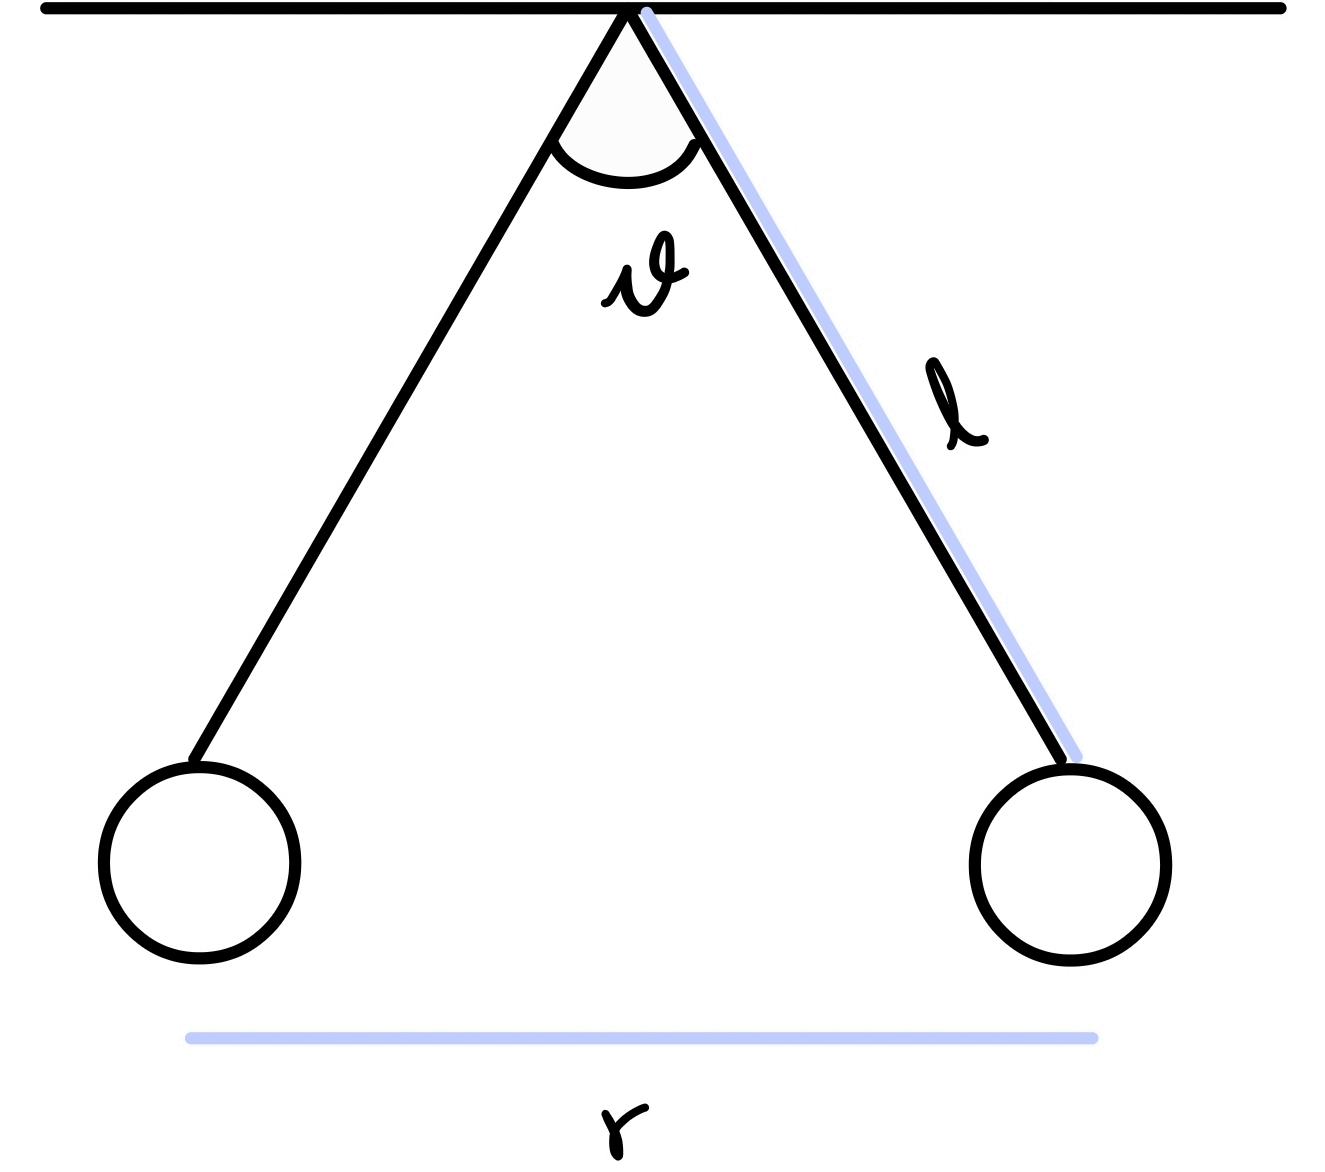
\includegraphics[width=6cm]{Diagrama3.png}
        \caption{Dos particulas puntuales con misma carga y masa, con un ángulo de separación $\theta$ debido a la Fuerza de Coulomb}
        \label{fig:xray}
        \end{center}
   \end{figure}\\
Sabemos que.
\begin{equation*}
    \sin\theta = \frac{\frac{r}{2}}{l} = \frac{r}{2l}
\end{equation*}
\begin{equation}
    \implies r = 2l \sin\theta
\end{equation}
Si ambas partículas se encuentran bajo fuerzas en equilibrio, tenemos que, para una partícula:
\begin{equation*}
    \begin{array}{cc}
     \sum_i \Vec{F_i} = 0     \\
     \Vec{F_e} +  \Vec{W} +  \Vec{T} = 0  
    \end{array}
\end{equation*}
Estas son las tres fuerzas que actúan en una partícula (Fuerza de Coulomb, gravedad y la tensión de la cuerda. Separándola por componentes:
\begin{equation*}
\begin{array}{cc}
    F_x = 0 & F_y = 0 \\
    F_x = T_x - F_e = 0& F_y = T_y - mg = 0   \\
    F_x = T\cos\theta - \Vec{F_e} = 0& T_y = mg \\  
\end{array}    
\end{equation*}
\begin{equation}
    \begin{array}{cc}
    T\cos\theta = F_e & T\cos\theta = mg \\
    \end{array}
\end{equation}
Sabemos que $F_e$ es la fuerza de Coulomb, que está dada por las ecuación (1) Y como la carga es la misma, se reescribe de la forma
\begin{equation*}
    F_{e}=k\frac{q^2}{r^2}
\end{equation*}
Volviendo a la ecuación (4).
\begin{equation*}
    \begin{array}{cc}
       T\cos\theta = F_e \\
       mg\cos\theta = k\frac{q^2}{r^2} \\
       q = r \sqrt{\frac{mg\sin\theta}{k}} \\
    \end{array}
\end{equation*}
y por la ecuación (2) tenemos la carga de la partícula:
\begin{equation}
    q = 2l\sin\theta\sqrt{\frac{mg\tan\theta}{k}}
\end{equation}

Un electroscopio es un instrumento que nos permite visualizar la existencia de un campo electrico inducido por una partícula cargada (o un conjunto de ellas), mostrándonos ángulos que van aumentando linealmente en función de cuán cargado esté nuestro sistema.\\

\begin{figure}[h]
    \centering
    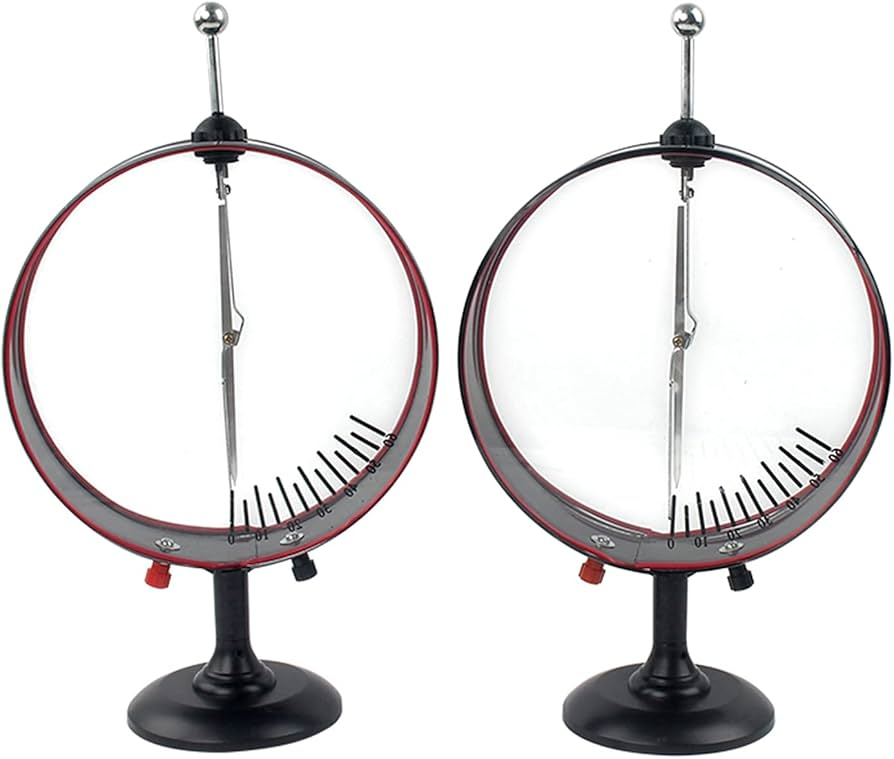
\includegraphics[width=0.5\linewidth]{Electroscope.png}
    \caption{Electroscopios con ausencia de carga.}
    \label{fig:enter-label}
\end{figure}

Esto nos será de gran utilidad pues este experimento consistirá en redistribuir las cargas de nuestro sistema frotando durante 30 segundos 10 diferentes tipos de tubos con 11 diferentes tipos de telas, comprendiendo tubos demasiado electropositivos tales como el bronce, latón, cobre hasta los más electronegativos como la madera, vidrio y acrílico. Asímismo, telas que son conocidas por cargar fácilmente los objetos como la lana y telas que carecen de estas propiedades, como la manta.\\
Por otro lado, al suministrar voltaje directamente al electroscopio mediante una fuente de poder debe influir en la posición de la manecilla de este, lo cual podría utilizarse para asocial voltaje a la carga que generó cada combinación de telas.\\\\

\subsection{Hipótesis}
Creémos que en cuanto a las telas será la lana, piel de conejo y polar las que carguen con mayor facilidad e intensidad a los tubos, particularmente al de vidrio, plástico y posiblemente el PVC, mostrando demasiada atracción la pelotita del péndulo hacia nuestra barra, del mismo modo el electroscopio mostrará un mayor ángulo al ser estas barras cargadas acercadas a su cabeza metálica; para nuestra segunda fase tener una idea intuitiva de cuanto voltaje logrará aumentar en $5^{\circ}$ la posición del electroscopio es demasiado complejo por lo que nos encantaría descubrirlo.\\
En la tercera fase del experimento esperamos un comportamiento similar al primero, viendo que al poner nuestro tubo cargado en medio de las dos bolas de unicel estas serán repelidas por un ángulo bastante amplio.\\

\subsection{Objetivos}
Al ver todas las posibles combinaciones en una tabla de 11 filas y 10 columnas (telas y tubos), y registrar de cuanto fue el ángulo de separación al acercar el tubo cargado, determinaremos cuales son las combinaciones que nos proporcionan cargas de mayor magnitud y si estas coinciden con nuestra hipótesis inicial; paralelamente, al concluir nuestra segunda etapa del experimento (con la fuente de alto voltaje), asociaremos un voltaje con su ángulo reflejado en el espectroscopio, siendo estos finalmente comparados con el ángulo mostrado por cada combinación de telas y hacer un registro gráfico de este comportamiento.\\
Por último, registraremos de cuanto es el ángulo con el que se separan las dos bolas de unicel al acercar el tubo (previamente cargado) en el centro para inducir la misma carga a ambas, esto será con las 3 combinaciones de tubos y telas que deducimos que fueron las más fuertes en magnitud.

\section{Desarrollo Experimental / Métodos}
Esta práctica consta de tres etapas
    \subsection{Etapa 1:}
    Material utilizado:
    \begin{itemize}
        \item Barras de distintos materiales: PVC, latón, madera, ebonita, aluminio, acrílico, teflón, plástico, cobre.
        \item Telas: Licra, licra con algodón, Tela polar, seda, terciopelo, razo, lana, franela, conejo, manta, chifón 
        \item 1 Soporte universal
        \item 1 Electroscopio
        \item 1 Hilo de algodon
        \item 1 Bola de unicel cubierta de aluminio
        \item 1 Nuez
        \item 1 barra de metal
        \item 1 pinza de tres dedos
    \end{itemize}
    En la primera etapa se montó un péndulo para la bola de unicel como se muestra en el diagrama.
    \begin{figure}[!tbh]
        \begin{center}
        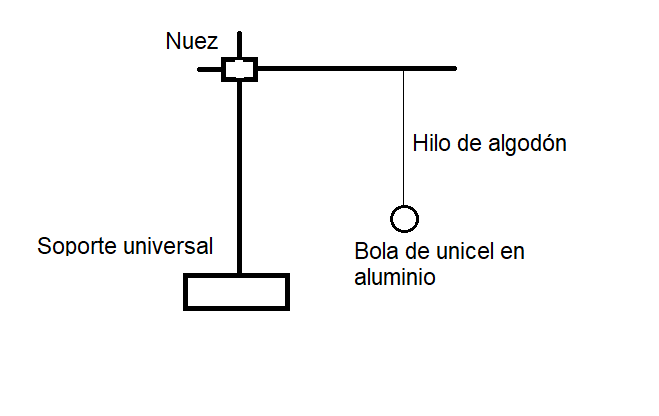
\includegraphics[width=11cm]{Diagrama1.png}
        \caption{Diagrama de la primera parte}
        \label{fig:xray}
        \end{center}
   \end{figure}
    Luego se frotó una barra con alguna tela, y una vez cargada, se le acercó a la bola de unicel y al electroscopio, pero sin llegara  tocarlos.
    Esto se repitió para todas las telas y las barras, haciendo todas las combinaciones posibles
    \subsection{Etapa 2:}
    Material utilizado:
    \begin{itemize}
        \item Fuente de alto voltaje
        \item Electroscopio
    \end{itemize}
    Tomamos la fuente de alto voltaje y construimos el arreglo conforme el manual nos indicaba, conectando los cables positivo y negativo, siendo la conexión a tierra sin ocupar pues no se nos otorgó este cable, la parte positiva de la fuente de alto voltaje fue conectada con la cabeza de metal del electroscopio mientras que la parte negativa fue conectada por un tornillo en la parte inferior del electroscopio, véase Figura 4 para entender mejor este arreglo.\\
    \begin{figure}[h]
        \centering
        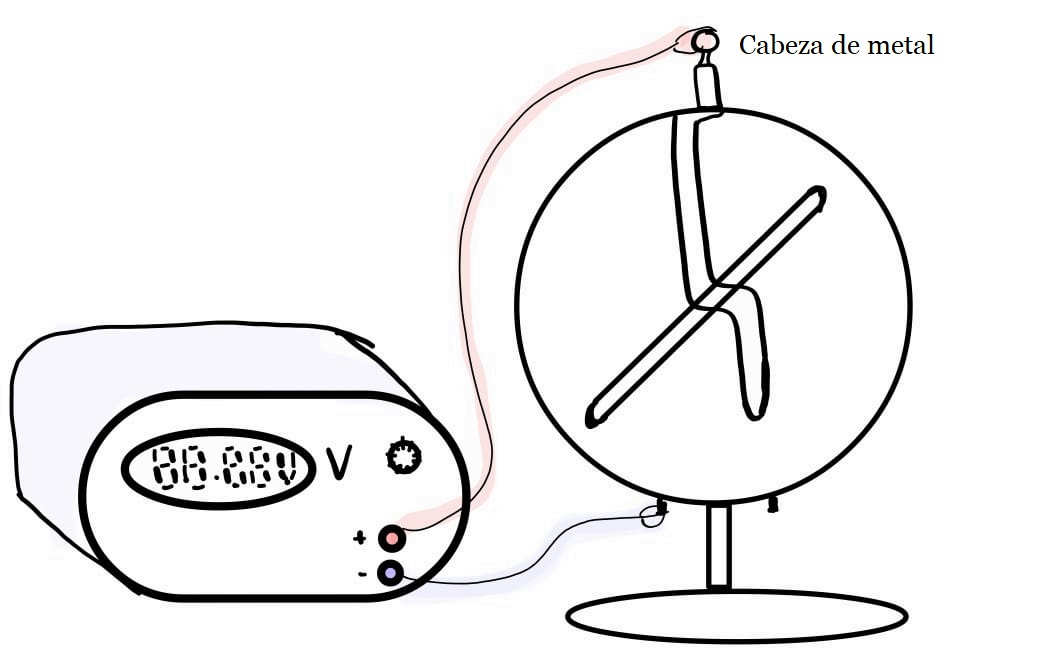
\includegraphics[width=0.5\linewidth]{Electroscope Arr Diagram.jpg}
        \caption{Electroscopio conectado a la fuente de alto voltaje}
    \end{figure}\\
En nuestro caso la fuente estaba en kV con mínima escala de 0.1kV; un miembro del equipo se colocó los guantes aislantes para manipular la fuente y procedimos a encenderla, fuimos incrementando muy lentamente el voltaje suministrado hasta ver que se cumplieran los primeros 5 grados, anotamos cuanto voltaje se requirió y se repitió el proceso. Esto se repitió hasta llegar a los $55^{\circ}$.
    
    \subsection{Etapa 3:}
    Material utilizado:
    \begin{itemize}
        \item Barras de distintos materiales: PVC, latón, madera, ebonita, aluminio, acrílico, teflón, plástico, cobre.
        \item Telas: Licra, licra con algodón, Tela polar, seda, terciopelo, razo, lana, franela, conejo, manta, chifón 
        \item 1 Soporte universal
        \item 2 Hilos de algodón
        \item 2 Bolas de unicel cubierta de aluminio pequeñas del mismo tamaño
        \item 1 Nuez
        \item 1 Barra de metal
        \item 1 Balanza
        \item 1 Flexómetro
        \item 1 Transportador
    \end{itemize}
    Para finalizar, se montó un doble pendulo sobre la barra como se muestra en el diagrama.
    \begin{figure}[!tbh]
        \begin{center}
        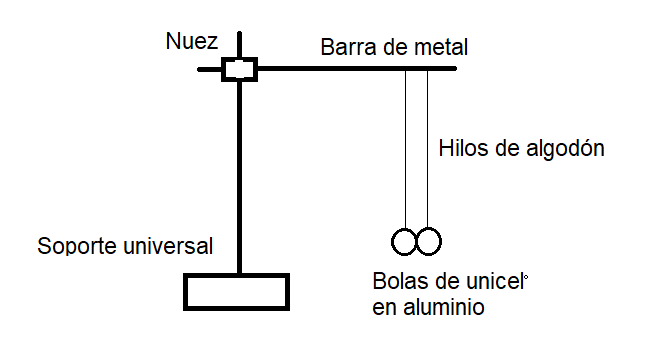
\includegraphics[width=11cm]{Diagrama2.png}
        \caption{Diagrama de la tercera parte}
        \label{fig:xray}
        \end{center}
   \end{figure}
   Ya teniendo registradas las combinaciones (hechas en la primera parte de la práctica), se eligen las 3 combinaciones con las que se registró más carga al frotarlos. Se vuelven a frotar esas 3 combinaciones para acercar  las barras, ya cargadas, a las bolas de unicel. Esto se hace por debajo de las bolas para que que carguen con el mismo signo lo mas cerca posible, por inducción, pero sin llegar a tocar la barra con alguna de las bolas, pues esto causaría que la carga se redistribuyera sobre todo el aluminio de manera uniforme (pues el alumino es un conductor). Luego se mide el ángulo de separación entre los hilos al separarse.

   También se registran las masas de las bolas de unicel, que deben ser lo más pequeñas e idénticas posibles (en tamaño y en masa).
\section{Resultados y discusión}
Hemos realizado un análisis cualitativo previamente al uso del electroscopio en el que obtuvimos la siguiente escala puntuando del 1 al 10.5 el grado de magnitud de desplazamiento.\\

\begin{figure}[h]
    \centering
    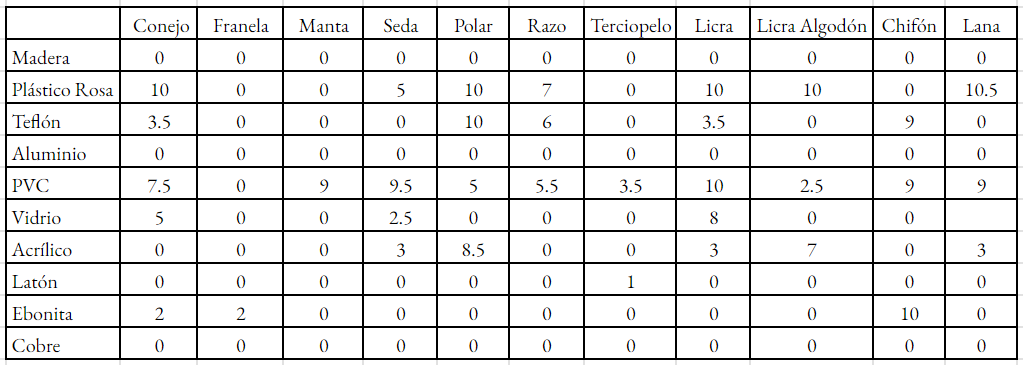
\includegraphics[width=1\linewidth]{Análisis Cualitativo.png}
    \caption{Análisis Cualitativo}
    \label{fig:enter-label}
\end{figure}\\

Esto nos muestra qué objetos distribuyen mejor la carga por su superficie, y cuáles mantienen la carga en el sitio en donde se frotó. A partir de esta tabla determinamos las mejores combinaciones, y usamos tres de ellas para la etapa 3 del experimento.

A continuación se muestra qué ángulo indicó el electroscopio al inducirle cada distinta carga con cada una de las combinaciones tela-tubo. Aquellos que fueron resaltados son los que presentaron la mayor cantidad de carga. \\
\begin{figure}[H]
    \centering
    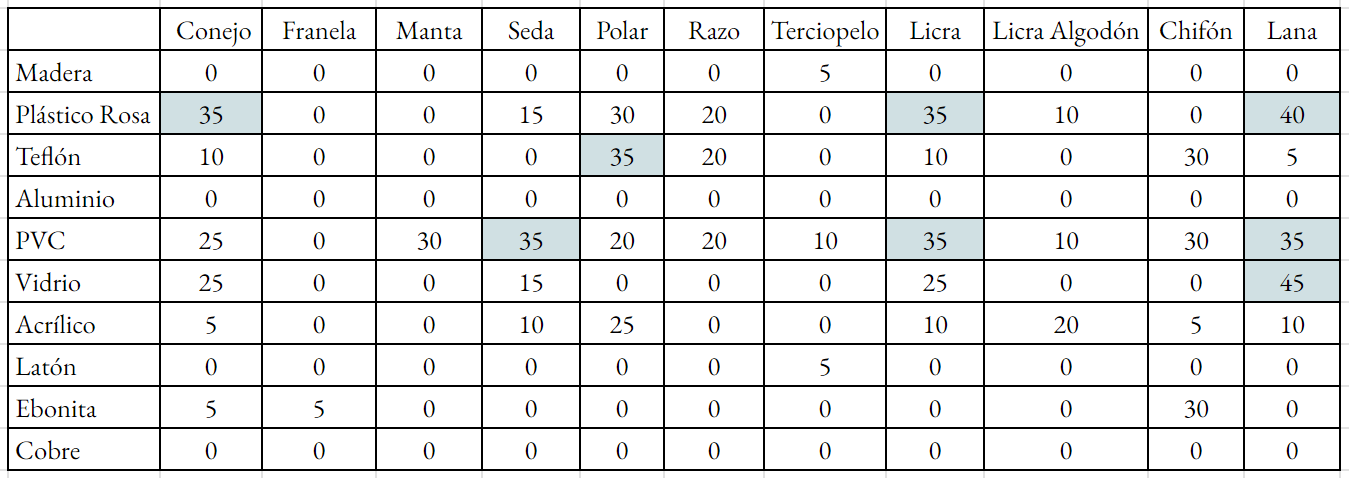
\includegraphics[width=1\linewidth]{Angulo.png}
    \caption{Ángulo mostrado en el electroscopio}
\end{figure}\\

Muestra una relación medianamente buena el análisis cualitativo con el cuantitativo, sin embargo es resaltable decir que tuvimos que hacer los 110 casos en el análisis cualitativo nuevamente pues en la primera ocasión a quien le asignamos el 10 fue rebasado por mucho en mediciones posteriores por lo que se ajustó el 10 al que vimos mejor en ese momento (lana con plástico rosa), pero a lo largo de las mediciones notamos que la lana con vidrio presentó un ligero pero notorio mayor movimiento al acercar el tubo, por lo que este nuevamente aumentó la escala, siendo ahora del 0 al 10.5; es rescatable que el análisis cualitativo a pesar de ser apoyado por una cámara celular y transportador es demasiado mal método. \\

Los datos para la fuente de alto voltaje en relación con el espectroscopio han sido los siguientes.

\begin{center}
\begin{table}[h]
\begin{tabular}{@{}cc@{}}
\toprule
kV                                 & \textbf{Ángulo} \\ \midrule
\multicolumn{1}{c|}{1.1 ± 0.05 kV}  & 5 ± 2.5°         \\
\multicolumn{1}{c|}{1.5 ± 0.05 kV}  & 10 ± 2.5°        \\
\multicolumn{1}{c|}{1.7 ± 0.05 kV}  & 15 ± 2.5°        \\
\multicolumn{1}{c|}{2.0 ± 0.05 kV}  & 20 ± 2.5°        \\
\multicolumn{1}{c|}{2.4 ± 0.05 kV} & 25 ± 2.5°        \\
\multicolumn{1}{c|}{2.9 ± 0.05 kV}  & 30 ± 2.5°        \\
\multicolumn{1}{c|}{3.2 ± 0.05 kV}  & 35 ± 2.5°        \\
\multicolumn{1}{c|}{3.7 ± 0.05 kV}  & 40 ± 2.5°        \\
\multicolumn{1}{c|}{4.5 ± 0.05 kV}  & 45 ± 2.5°        \\
\multicolumn{1}{c|}{5.6 ± 0.05 kV}   & 50 ±2 .5°        \\
\multicolumn{1}{c|}{6.1 ± 0.05 kV}                    & 55 ±2.5°        \\ \bottomrule
\end{tabular}
\end{table}
\end{center}\\

Esta por lo que nos dice la teoría no es una relación lineal, es demostrado al intentar graficar y aplicar ecuaciones de la regresión lineal en donde el resultado es fatal. Según la teoría nos indica que la relación Ángulo vs Voltaje es mediante una raíz cuadrada (A vs $\sqrt{V}$). Es entonces que al graficar A vs $\sqrt{V}$, aplicar la regresión lineal, revertir la trasformación y expresarla en una función A vs V obtenemos la siguiente gráfica y relación (la zona azul es el rango de incertidumbre).\\
\begin{figure}[h]
    \centering
    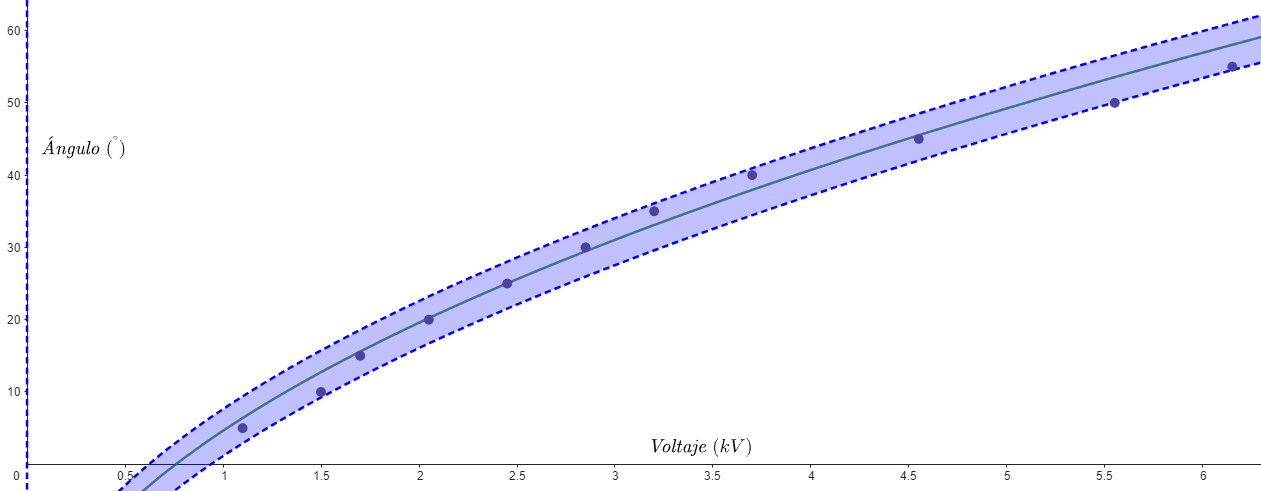
\includegraphics[width=1\linewidth]{Avsr(V).png}
    \caption{Gráfica Ángulo ($^{\circ}$) vs Voltaje (kK)}
    \label{fig:enter-label}
\end{figure}\\

Finalmente, utilizando la ecuación (5) obtuvimos la carga que debían tener las bolas de unicel en aluminio.\\
    \begin{figure}[h]
        \begin{center}
        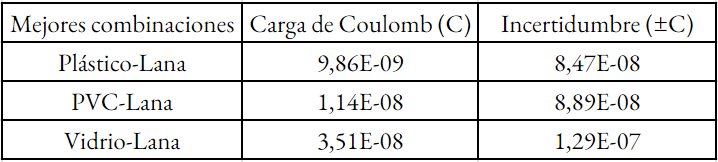
\includegraphics[width=11cm]{Cargas con incertidumrbes.png}
        \caption{Cargas de las bolas de unicel cubiertas en aluminio, resultantes de cargar por inducción con las combinaciones Plástico-Lana, PVC-Lana, Vidrio-Lana}
        \label{fig:xray}
        \end{center}
   \end{figure}\\
Estos resultados nos muestran la carga que pueden llegar a tener los objetos que más afinidad tuvieron al cargarse por frotamiento. A pesar de que los ángulos no eran demasiado grandes, si se logra diferenciar entre el objeto que obtuvo mayor carga.\\\\

Por último, obtener qué relación tiene el ángulo con el voltaje nos permitió colocar en la gráfica a las 3 combinaciones más poderosas en cuestión de carga y asociar un voltaje.\\

\begin{figure}
    \centering
    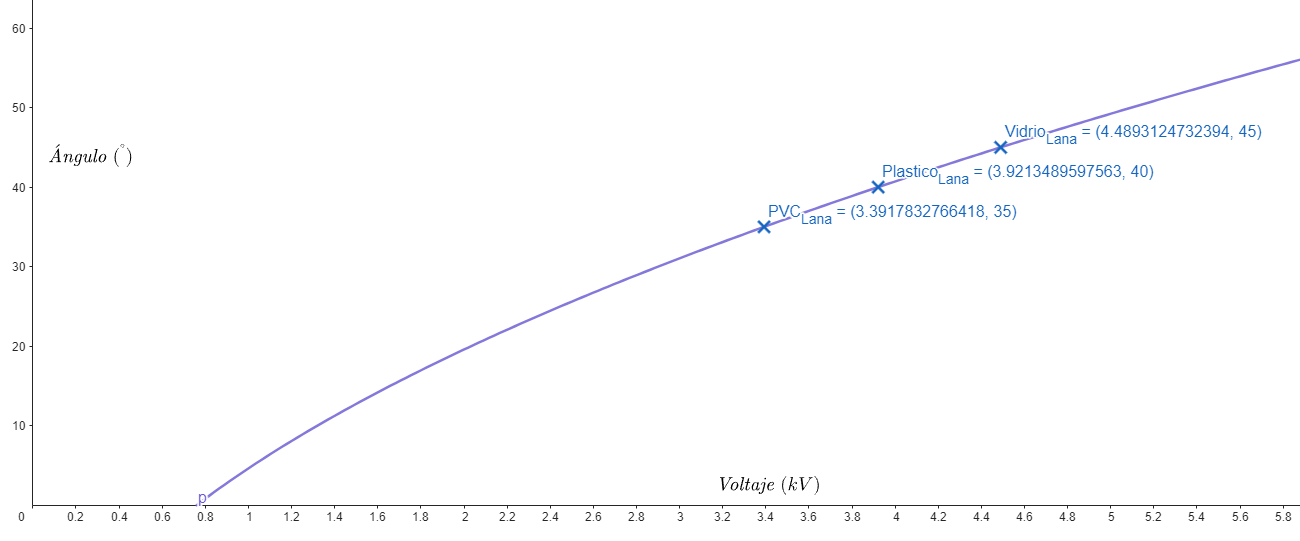
\includegraphics[width=1\linewidth]{Colocacion.png}
    \caption{Colocación aparente de las combinaciones con un voltaje.}
    \label{fig:enter-label}
\end{figure}
\section{Conclusiones}
A partir de la Tabla en la Figura 7. podemos deducir que los objetos que más se cargaban por frotación eran el plástico rosa, el PVC, el teflón y el vidrio. La efectividad de cargar esos objetos aumentaba mucho con la seda, la licra, la tela polar y de conejo. Pero la tela que destacó fue la lana.
Ya con esto pudiendo deducir y elegir las mejores combinaciones que fueron:  Plástico-Lana, PVC-Lana y Vidrio-Lana.
\\ 
Para la segunda etapa, la gráfica muestra un comportamiento muy similar al de la gráfica de $\sqrt{x}$ esto coincide con el razonamiento mostrado en los resultados, pues en efecto no muestra un comportamiento lineal y los puntos en la distribución solo muestran una pequeña variación.
\\ 
Por último, para la tercera etapa tenemos la tabla de la figura 9. Se observa que la carga calculada de las tres combinaciones mostradas coinciden en orden de magnitud con las obtenidas en la etapa 1. Siendo la combinación de Vidrio-Lana la que más afinidad tuvo para cargarse por frotamiento.
\\
El desarrollo (teórico y experimental) fue capaz de predecir el comportamiento de los materiales y las relaciones entre ellos.\\\\

\newpage
\noindent {\bf Declaración de contribución de los autores}\\ 

Iván Bautista Alvarado$^1$ y Andrés López González$^1$ hemos realizado tanto el apartado escrito como el análisis de manera colectiva siendo una participación del 100\% por parte de ambos y no solo una repartición.\\ 

{\bf Agradecimientos} \\ 

A ese.\\

\begin{figure}[h]
    \centering
    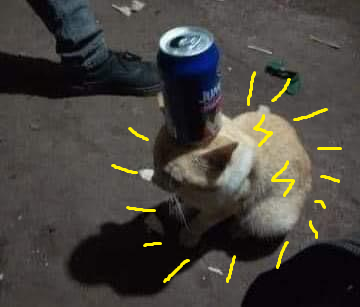
\includegraphics[width=0.5\linewidth]{el.png}
    \caption{Electrogato}
    \label{fig:enter-label}
\end{figure}\\

\begin{thebibliography}{99}

\bibitem{griffiths}
D. J. Griffiths, \textit{Introduction to Electrodynamics}, 3rd ed. Upper Saddle River, NJ, USA: Prentice-Hall, 1999.

\bibitem{jackson}
J. D. Jackson, \textit{Classical Electrodynamics}, 3rd ed. New York, NY, USA: Wiley, 1998.

\bibitem{sadiku}
M. N. O. Sadiku, \textit{Elements of Electromagnetics}, 6th ed. New York, NY, USA: Oxford University Press, 2014.

\bibitem{wangsness}
R. K. Wangsness, \textit{Electromagnetic Fields}, 2nd ed. New York, NY, USA: Wiley, 1986.

\bibitem{zangwill}
A. Zangwill, \textit{Modern Electrodynamics}. Cambridge, UK: Cambridge University Press, 2013.

\bibitem{purcell}
E. M. Purcell and D. J. Morin, \textit{Electricity and Magnetism}, 3rd ed. Cambridge, UK: Cambridge University Press, 2013.

\bibitem{shadowitz}
A. Shadowitz, \textit{The Electromagnetic Field}. Mineola, NY, USA: Dover Publications, 1988.


\end{thebibliography}


\end{document}